\documentclass[10pt,a4paper]{article}
\usepackage[czech]{babel}
\usepackage[utf8]{inputenc}
\usepackage{graphicx}
\usepackage{amsfonts}
\usepackage{hhline}
\usepackage{hyperref}
\usepackage{placeins}
\usepackage{amssymb}
\newcommand{\footer}{{\small\em Mám něco špatně? Otevři PR na \href{https://github.com/kosciCZ/MAT-GF}{Githubu}!}}
\begin{document}
\bfseries\noindent4) (15b) Napište tabulku operace násobení (druhá skupina měla sčítání) v $GF(4)$. Jako ireducibilní  polynom použijte $x^2 + x + 1$ a prvky tělesa $GF(4)$ vyjádřete v tabulce jako vektory se souřadnicemi v bázi $\lbrace 1,\alpha \rbrace$, kde $\alpha$ je primitivní prvek. (druhá skupina měla jako mocniny primitivního prvku).\normalfont
 \footer
\subsection*{Postup řešení:}
\subsubsection*{Výpočet primitivních prvků $\alpha$}
Nejdříve je nutno odvodit počet prvků, neboli to v jaké zbytkové třídě se nacházíme. GF($2^{2}$) nám značí zbytkovou třídu $\mathbb{Z}_{4}$, tedy čtyři prvky celkem. Prvky GF jsou polynomy. Máme zadán generující polynom, pomocí kterého lze odvodit prvky tohoto pole. Řád generujícího polynomu vždy bude shodný s číslem $n$, na které je umocněna 2 v značení GF($2^{n}$). Číslo $n$ také značí počet bitů, na které se budou kódovat prvky pole.

\renewcommand{\arraystretch}{1.5}%
\begin{table}[h]
	\centering
	\begin{tabular}{|c|c|c|}
		\hline
		\textbf{Prvek} & \textbf{Notace polynomem} & \textbf{Binární kódování} \\\hline
		0 & 0 & 00 \\\hline 
		$\alpha^{0}$ &  1 & 01 \\\hline 
		$\alpha^{1}$ & $x\cdot\alpha^{0}=x$ & 10 \\\hline 
		$\alpha^{2}$ & $x\cdot\alpha^{1}=x^{2} = x + 1$ & 11 \\\hline 
	\end{tabular}
\end{table}

Binární kódování polynomu znamená pouze to, že pro i-tou mocninu x napíšeme 1 pokud tam je a 0 pokud tam není (např. $x^2 + x + 1 \to 111$, nebo $x^3 + 1 \to 1001$). Při vytváření prvků pole se vždy začíná nulou, a $\alpha^{0} = 1$. Každá další $\alpha^{i}$ se dá vypočítat jako $x\cdot\alpha^{i-1}$. V tabulce lze vidět takto vypočítanou $\alpha^{1}$, kterou lze pohodlně zakódovat na 2 bity. Problém nastává až s $\alpha^{2} = x^{2}$, což se na dva bity zakódovat nedá, na tři ale ano ($x^{2} \to 100$). Nyní je jen potřeba prvek dostat do pole, tedy ho XORovat s generujícím polynomem a oříznout na dva bity:
$$ 100 \oplus 111 = 011 $$
Což je po oříznutí $11$. Tabulka je tedy hotová, pokud bychom se pokusili o výpočet $\alpha^{3}$, dostali bychom opět $\alpha^{0}$.


\subsubsection*{2a) Tvorba tabulky pro operaci sčítání s mocninami $\alpha$}
Operace sčítání není v GF nic jiného než obyčejný XOR binární reprezentace. Pro tvorbu tabulky je jen pak potřeba najít odpovídající alfu. Pozor, v GF($2^{n}$) je operace sčítání stejná jako odčítání.
\begin{table}[h]
	\centering
	\begin{tabular}{|c||c|c|c|c|}
		\hline
		+ & 0& $\alpha^{0}$ & $\alpha^{1}$ & $\alpha^{2}$ \\\hhline{|==|=|=|=|}
		0 &  0 & $\alpha^{0}$ & $\alpha^{1}$ & $\alpha^{2}$ \\\hline 
		$\alpha^{0}$ & $\alpha^{0}$ & 0 & $\alpha^{2}$ & $\alpha^{1}$ \\\hline 
		$\alpha^{1}$ & $\alpha^{1}$ & $\alpha^{2}$ & 0 & $\alpha^{0}$ \\\hline 
		$\alpha^{2}$ & $\alpha^{2}$ & $\alpha^{1}$ & $\alpha^{0}$ & 0 \\\hline 
	\end{tabular}
\end{table}
\newpage
\subsubsection*{2b) Tvorba tabulky pro operaci násobení s vektory v bázi $\lbrace 1,\alpha \rbrace$}
Abych se přiznal, tak netuším, co znamenají ty vektory báze, ale podle vzorového řešení je to jen binární reprezentace s MSB vpravo, tedy opačně než jsem si zapsal nahoře do tabulky. \\\\
Násobení v GF(q) funguje tak, že $\alpha^{i}\cdot\alpha^{j} = \alpha^{(i+j) mod (q-1)}$.
V našem případě, tedy GF(4) např. $\alpha^{1}\cdot\alpha^{2} = \alpha^{3 mod 3} = \alpha^{0} \to 01$ binárně $\to (1,0)$ ve vektoru.
\begin{table}[h]
	\centering
	\begin{tabular}{|c||c|c|c|c|}
		\hline
		$\cdot$ & $(0,0)$& $(1,0)$ & $(0,1)$ & $(1,1)$ \\\hhline{|==|=|=|=|}
		$(0,0)$ & $(0,0)$ & $(0,0)$ & $(0,0)$ & $(0,0)$ \\\hline 
		$(1,0)$ & $(0,0)$ & $(1,0)$ & $(0,1)$ & $(1,1)$ \\\hline 
		$(0,1)$ & $(0,0)$ & $(0,1)$ & $(1,1)$ & $(1,0)$ \\\hline 
		$(1,1)$ & $(0,0)$ & $(1,1)$ & $(1,0)$ & $(0,1)$ \\\hline 
	\end{tabular}
\end{table}

\subsection*{Zdrojové materiály:}
\href{https://www.fit.vutbr.cz/study/courses/BMS/private/bms0x6_dvb.pdf}{Slidy k BMS (14,15)}

\begin{figure}[h!]
	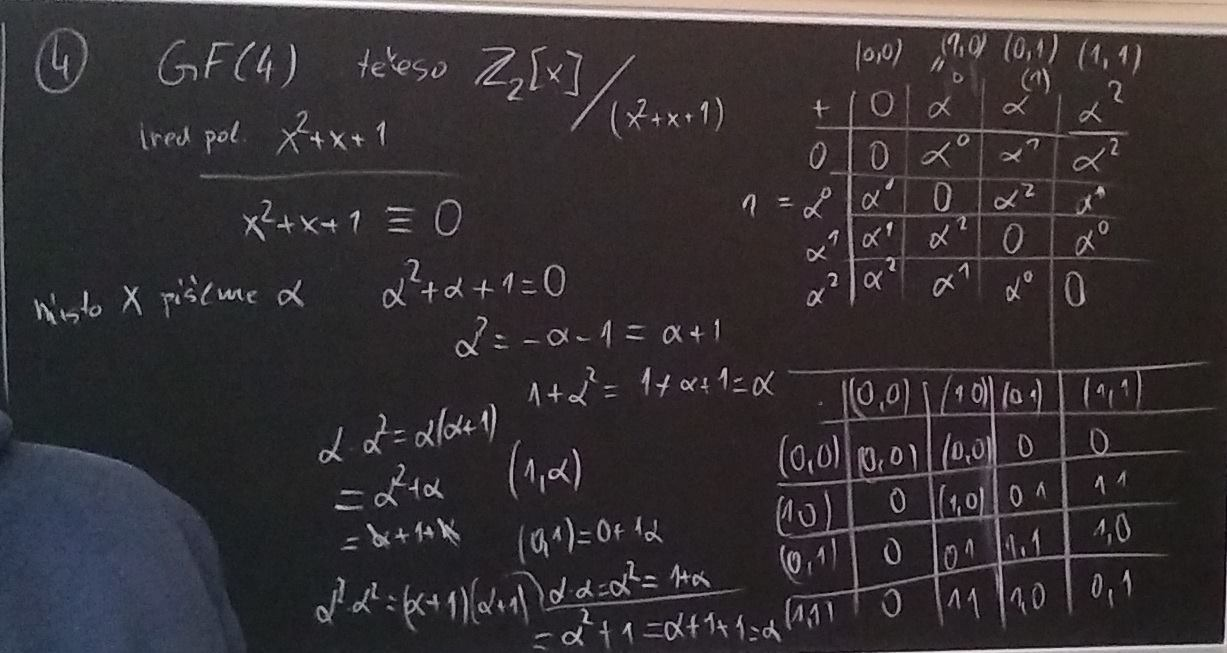
\includegraphics[width=\linewidth]{reseni}
	\caption{Vzorové řešení z konzultací}
	\label{graph:gprof}
\end{figure}
\FloatBarrier

\end{document}
